\chapter{3D打印建模}
\label{cha:Model}

\section{测试用3轮底盘}

需要考虑到电机和定位模块的配合。

定位模块外形为 $\phi$ 11.2 X 25.1mm,至少需要留12mm直径的圆柱形空间,头部距离地面不得超过2mm。定位模块外形尺寸如图~\ref{fig:Camera-Dimension}。

\begin{figure}[htbp]
    \centering
    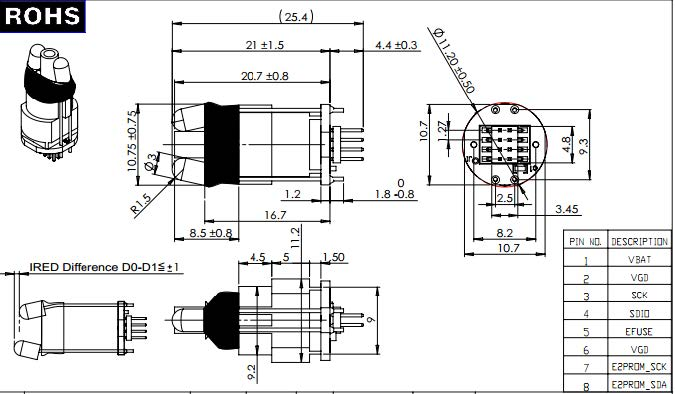
\includegraphics[width=\columnwidth]{SONIX_OID_SNM9S500C3000A_Specification_V1-Dimension.jpg}
    \caption{定位模块外形尺寸}
    \label{fig:Camera-Dimension}
\end{figure}

底盘图纸如图~\ref{fig:Assembled-Test-Datasheet}。

\begin{figure}[htbp]
    \centering
    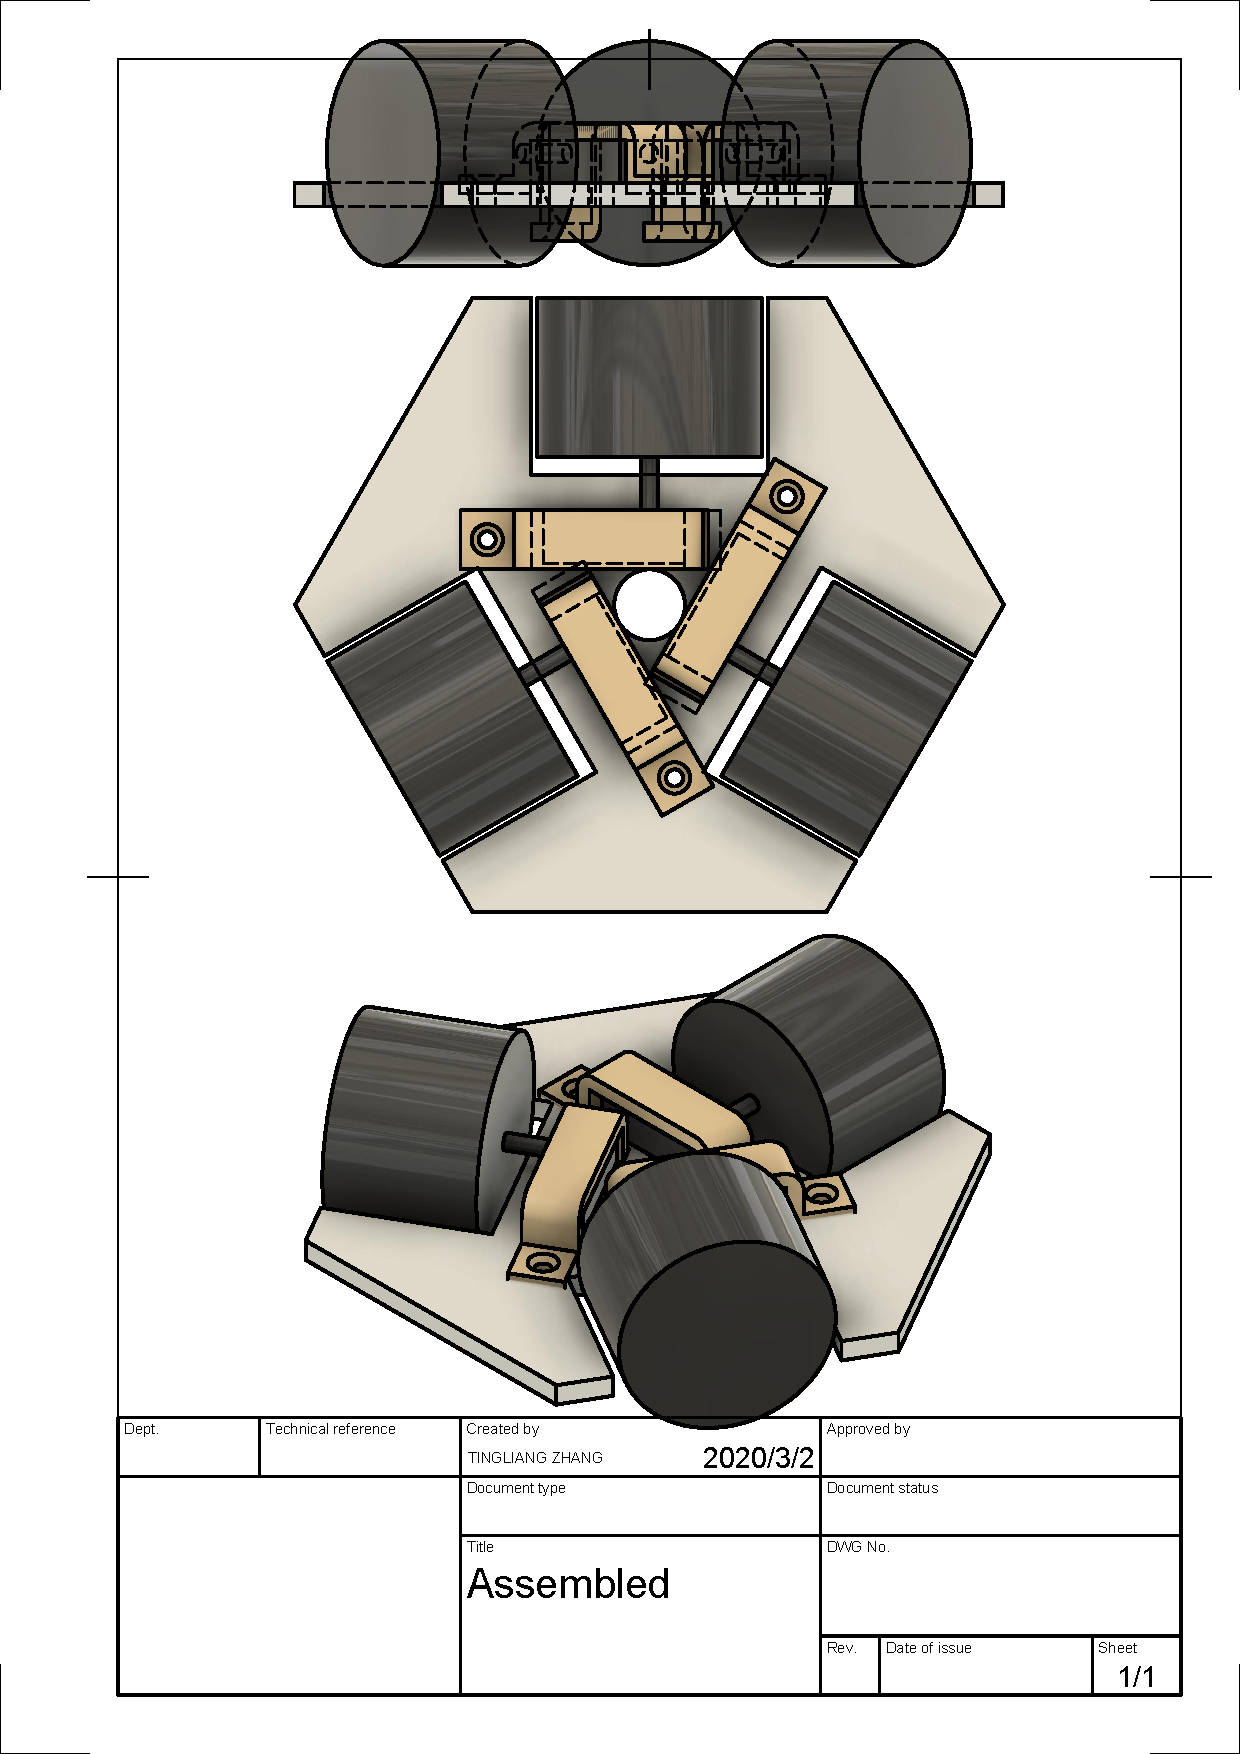
\includegraphics[width=\columnwidth]{Assembled-v1.pdf}
    \caption{测试用底盘图纸}
    \label{fig:Assembled-Test-Datasheet}
\end{figure}

测试用底盘渲染图如图~\ref{fig:Assembled-Test-Render}。

\begin{figure}[htbp]
    \centering
    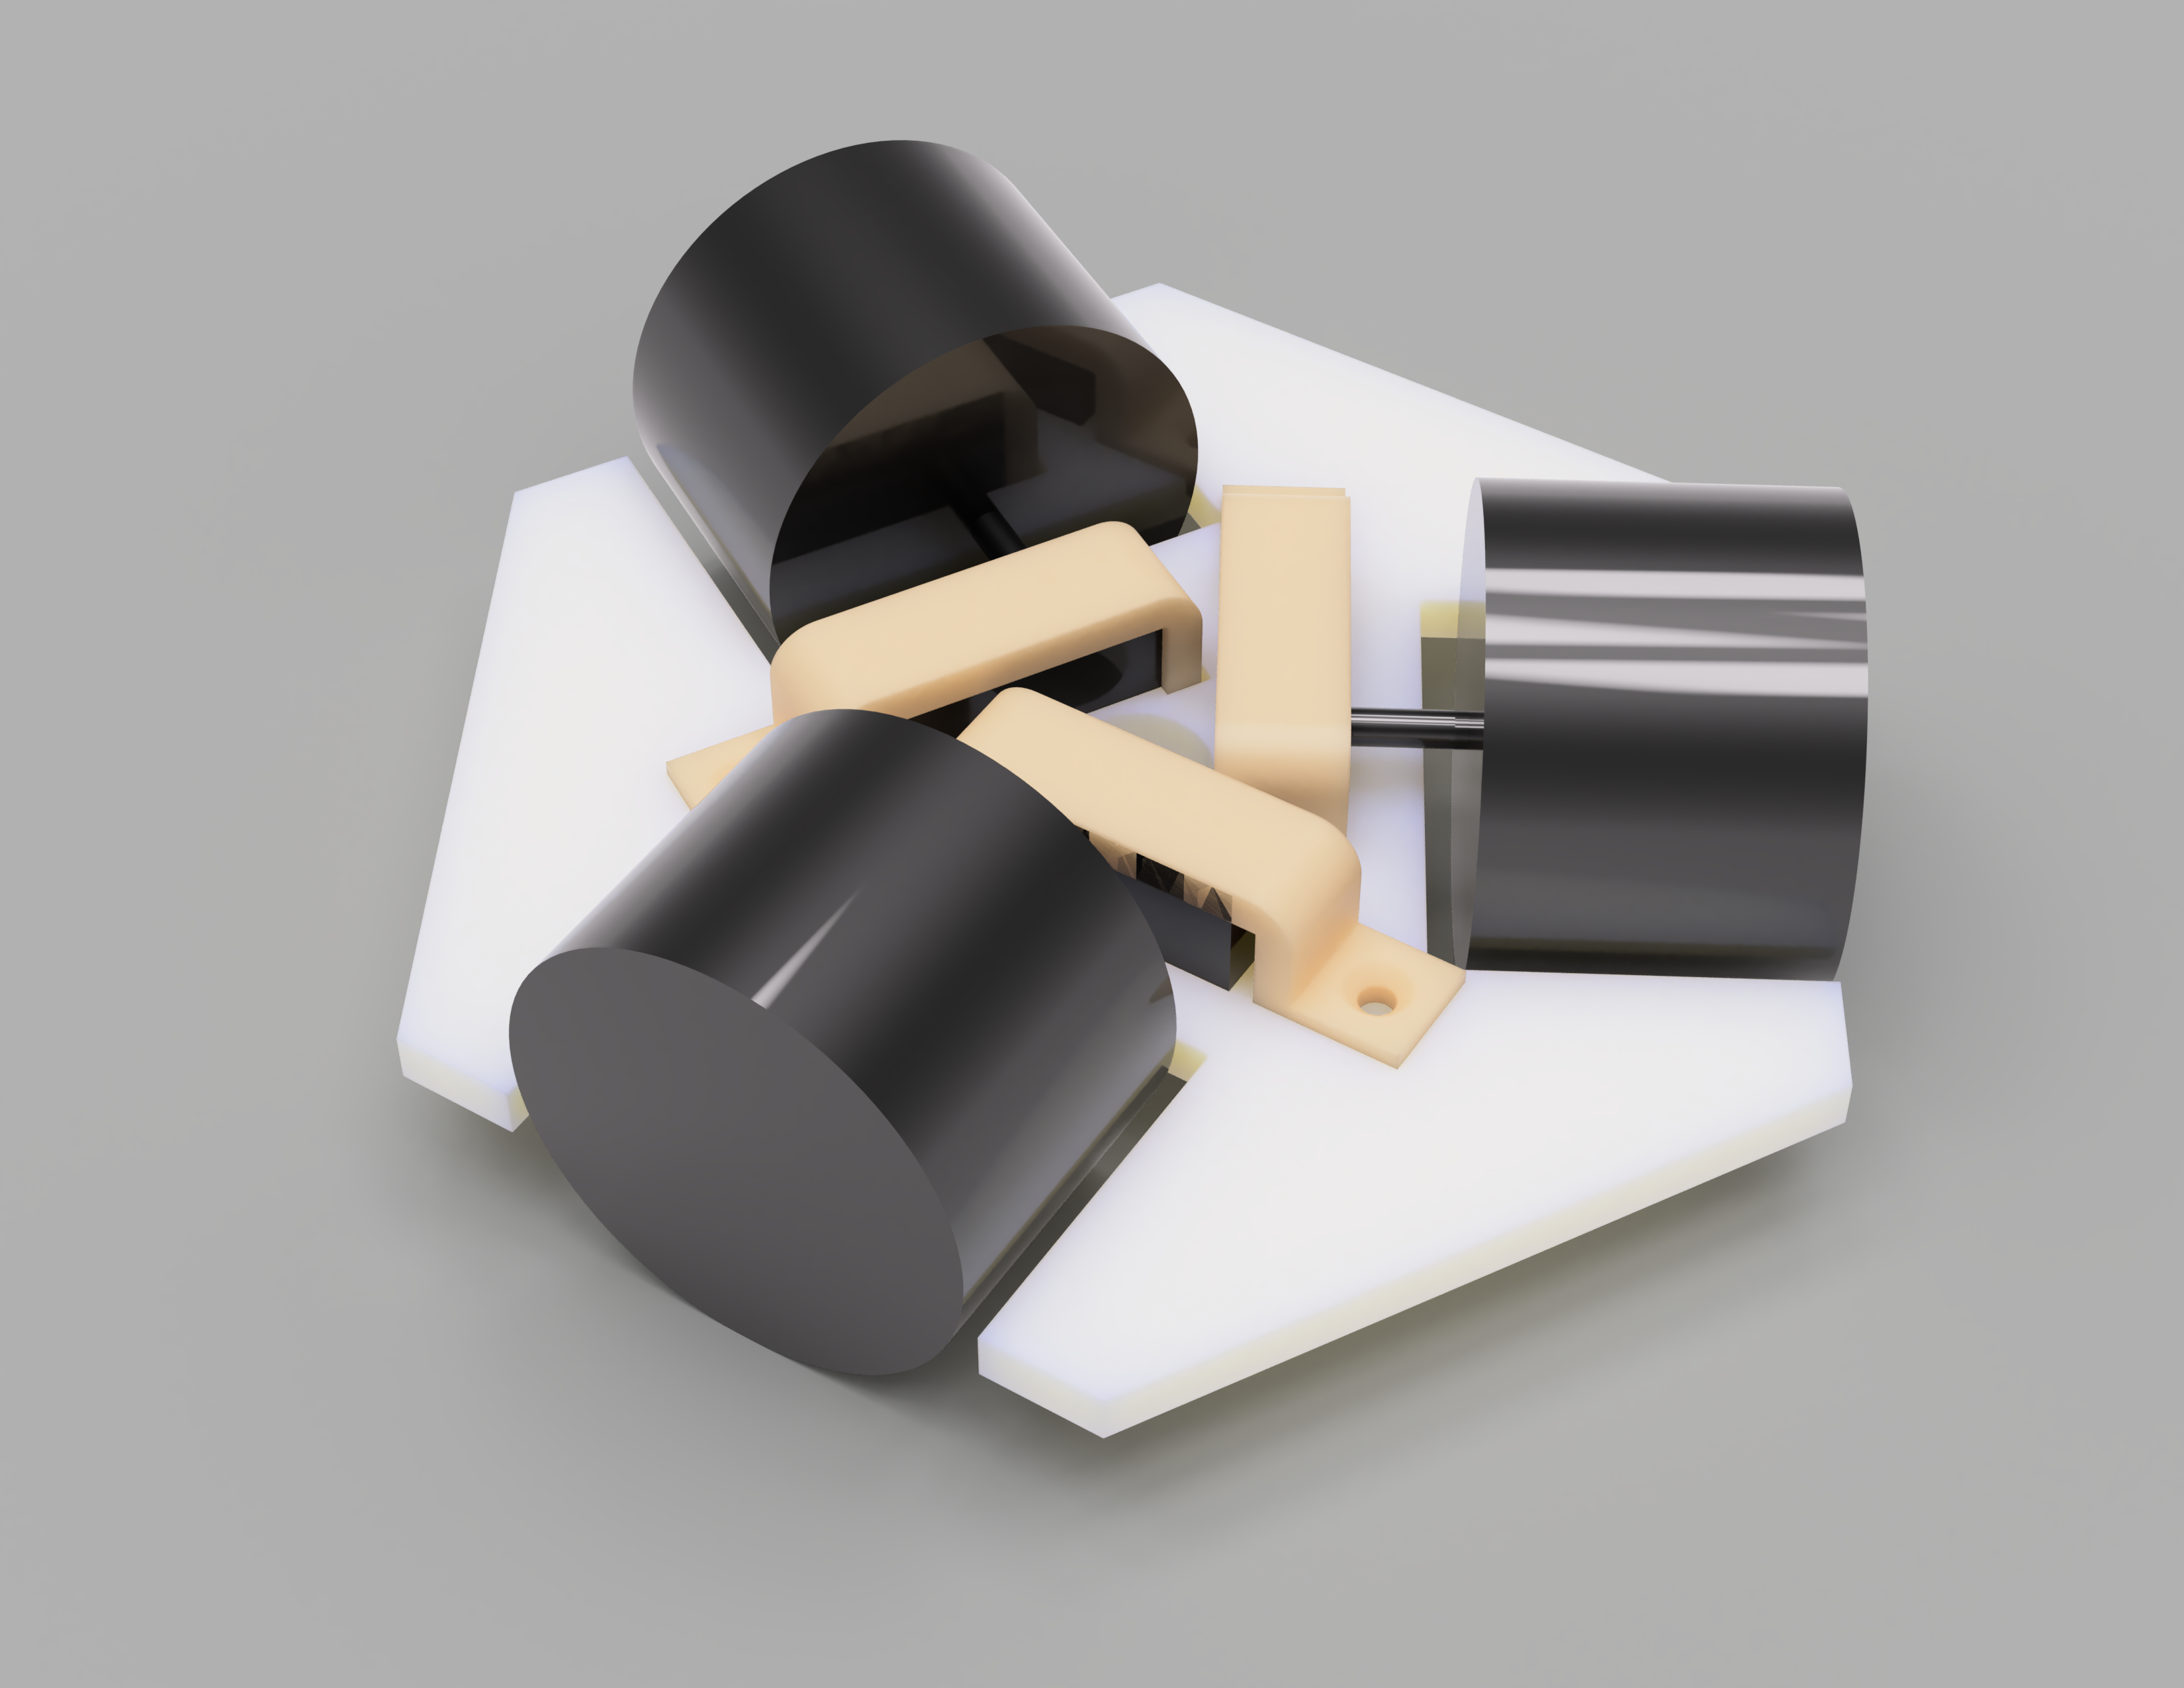
\includegraphics[width=\columnwidth]{Assembled_2020-Mar-02.png}
    \caption{测试用底盘渲染图}
    \label{fig:Assembled-Test-Render}
\end{figure}

其中,电机固定件使用的是一颗沉头M3*10的不锈钢螺栓。固定件上留出大径5.3mm小径3mm的沉头螺丝孔,底板上则留一个直径5.9mm圆内接正六边形深度为2.5mm的六角螺母固定孔,以便不用鸭嘴钳拧螺丝,当然也有3mm的圆孔。